\documentclass[11pt,a4paper]{article}

\newcommand{\tumsoTime}{09:00 น. - 12:00 น.}
\newcommand{\tumsoRound}{1}

\usepackage{../tumso}

\begin{document}

\begin{problem}{Space War 2}{standard input}{standard output}{1.5 seconds}{512 megabytes}{250}

ในศึกศักดิ์ศรีระหว่างทหารทั่วโลก 20th Tough Universe Military Struggle Olympic (TUMSO 20) ได้รับสปอนเซอร์จากเว็บไซต์หนึ่ง ให้จัดการแข่งขันขึ้นที่เมือง OTOK โดยสนามแข่งเป็นสนามที่ใหญ่มาก ซึ่งอยู่ในระนาบ 2 มิติ มีตึกติดกันอยู่ทั้งหมด $N$ ตึก ตึกที่ $i$ จะสูง $H_i$ หน่วยจากพื้นดิน และด้านบนตึกแต่ละตึกจะมีพื้นที่ที่สามารถวางป้อมลอยฟ้าได้ ซึ่งด้านบนตึกที่ $i$ จะสามารถวางป้อมได้ในช่วงความสูงตั้งแต่ $L_i$ ถึง $R_i$ จากพื้นดิน และด้านบนตึกแต่ละตึกจะสามารถวางป้อมได้ตึกละไม่เกิน 1 ป้อม

ป้อมแต่ละป้อมจะสามารถยิงขีปนาวุธได้ โดยขีปนาวุธนี้จะเคลื่อนที่ได้ในแนวขนานกับแกน X หรือ Y เท่านั้น และเมื่อยิงออกไปแล้วจะสามารถทำการเลี้ยวได้ไม่เกิน $1$ ครั้ง เนื่องจากตึกทั้ง $N$ ตึกทำจากไวเบรเนี่ยมจึงไม่สามารถยิงขีปนาวุธทะลุตึกได้

ในเมือง OTOK จะมียามผู้ซึ่งทำหน้าที่ดูแลความสงบของเมืองอยู่ ถ้าหากป้อมสองป้อมใด ๆ สามารถยิงขีปนาวุธใส่กันได้ จะทำให้เมืองไม่เกิดความสงบ ซึ่งยามไม่ต้องการเช่นนั้น จึงต้องการให้คุณหาจำนวนวิธีในการวางป้อมทั้งหมด (โดยสามารถวางจำนวนเท่าใด หรือไม่วางก็ได้) โดยเมื่อวางแล้วยังทำให้เมือง OTOK สงบสุขอยู่ แต่เนื่องจากคุณอยู่ในดินแดนอันห่างไกลจึงต้องส่งข้อความผ่านทางเครื่องส่งสาร ซึ่งสามารถส่งตัวเลขได้เพียง 9 หลัก ยามจึงให้คุณส่งเศษจากการหารจำนวนวิธีทั้งหมดด้วย $998244353$ แทน

\begin{center}
\parindent \resizebox{5cm}{!}{
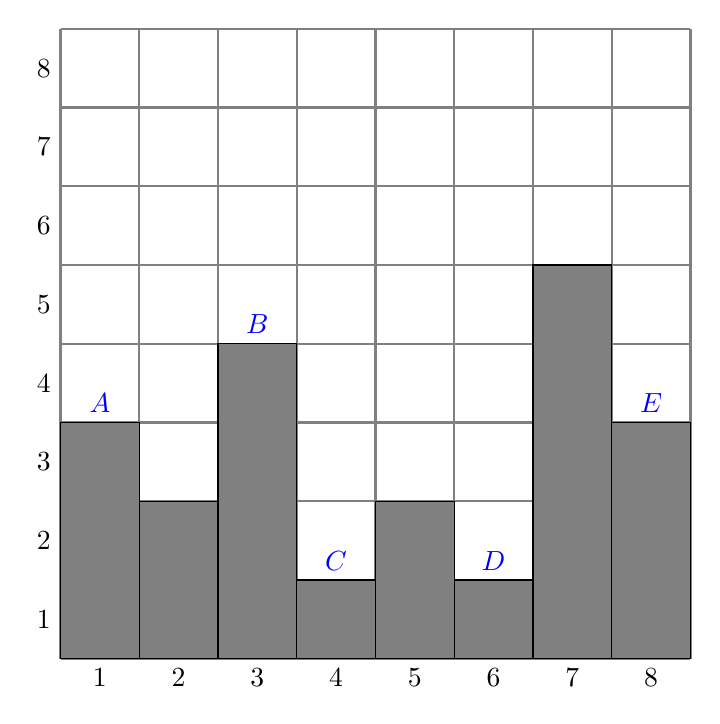
\begin{tikzpicture}
    \draw[step=1cm,gray,thick] (0.0,0.0) grid (8.0,8.0);
    
    \filldraw[black] (0.5,0) circle (0pt) node[anchor=north]{$1$};
    \filldraw[black] (1.5,0) circle (0pt) node[anchor=north]{$2$};
    \filldraw[black] (2.5,0) circle (0pt) node[anchor=north]{$3$};
    \filldraw[black] (3.5,0) circle (0pt) node[anchor=north]{$4$};
    \filldraw[black] (4.5,0) circle (0pt) node[anchor=north]{$5$};
    \filldraw[black] (5.5,0) circle (0pt) node[anchor=north]{$6$};
    \filldraw[black] (6.5,0) circle (0pt) node[anchor=north]{$7$};
    \filldraw[black] (7.5,0) circle (0pt) node[anchor=north]{$8$};
    % \filldraw[black] (8.5,0) circle (0pt) node[anchor=north]{$9$};

    \filldraw[black] (0,0.5) circle (0pt) node[anchor=east]{$1$};
    \filldraw[black] (0,1.5) circle (0pt) node[anchor=east]{$2$};
    \filldraw[black] (0,2.5) circle (0pt) node[anchor=east]{$3$};
    \filldraw[black] (0,3.5) circle (0pt) node[anchor=east]{$4$};
    \filldraw[black] (0,4.5) circle (0pt) node[anchor=east]{$5$};
    \filldraw[black] (0,5.5) circle (0pt) node[anchor=east]{$6$};
    \filldraw[black] (0,6.5) circle (0pt) node[anchor=east]{$7$};
    \filldraw[black] (0,7.5) circle (0pt) node[anchor=east]{$8$};
    % \filldraw[black] (0,8.5) circle (0pt) node[anchor=east]{$9$};

    \filldraw[fill=gray, draw=black] (0,0) rectangle (1,3);
    \filldraw[fill=gray, draw=black] (1,0) rectangle (2,2);
    \filldraw[fill=gray, draw=black] (2,0) rectangle (3,4);
    \filldraw[fill=gray, draw=black] (3,0) rectangle (4,1);
    \filldraw[fill=gray, draw=black] (4,0) rectangle (5,2);
    \filldraw[fill=gray, draw=black] (5,0) rectangle (6,1);
    \filldraw[fill=gray, draw=black] (6,0) rectangle (7,5);
    \filldraw[fill=gray, draw=black] (7,0) rectangle (8,3);
    
    \filldraw[black] (0.5,3) circle (0pt) node[anchor=south]{\textcolor{blue}{$A$}};
    \filldraw[black] (2.5,4) circle (0pt) node[anchor=south]{\textcolor{blue}{$B$}};
    \filldraw[black] (3.5,1) circle (0pt) node[anchor=south]{\textcolor{blue}{$C$}};
    \filldraw[black] (5.5,1) circle (0pt) node[anchor=south]{\textcolor{blue}{$D$}};
    \filldraw[black] (7.5,3) circle (0pt) node[anchor=south]{\textcolor{blue}{$E$}};
\end{tikzpicture}
} 
\end{center}

จากภาพถ้าวางป้อมลอยฟ้าที่ตำแหน่ง \textcolor{blue}{$A$}, \textcolor{blue}{$C$} หรือ \textcolor{blue}{$A$}, \textcolor{blue}{$D$} หรือ \textcolor{blue}{$A$}, \textcolor{blue}{$E$} หรือ \textcolor{blue}{$B$}, \textcolor{blue}{$E$} หรือ \textcolor{blue}{$C$}, \textcolor{blue}{$D$} หรือ \textcolor{blue}{$C$}, \textcolor{blue}{$E$} หรือ \textcolor{blue}{$D$}, \textcolor{blue}{$E$} จะยังคงสงบอยู่ แต่ถ้าวางป้อมลอยฟ้าที่ตำแหน่ง \textcolor{blue}{$A$}, \textcolor{blue}{$B$} หรือ \textcolor{blue}{$B$}, \textcolor{blue}{$C$} หรือ \textcolor{blue}{$B$}, \textcolor{blue}{$D$} จะเกิดความไม่สงบ

\InputFile
ข้อมูลนำเข้ามีทั้งหมด $Q+1$ บรรทัด

บรรทัดแรกประกอบด้วยจำนวนเต็ม $N$ แทนจำนวนตึกทั้งหมดในเมือง OTOK $(1\leq N\leq 10^{5})$

บรรทัดที่ $2$ ประกอบด้วยจำนวนเต็ม $N$ จำนวน คือ $H_1,H_2,\ldots,H_N$ โดยที่ $H_i$ แทนความสูงของตึกที่ $i$ $(0\leq H_i<10^5)$

บรรทัดที่ $3$ ถึง $N+2$ ประกอบด้วยจำนวนเต็ม $2$ จำนวน คือ $L_i$ และ $R_i$ แทนตำแหน่งของพื้นที่ที่ป้อมลอยฟ้าสามารถวางได้ $(H_i<L_i\leq R_i\leq 10^5)$

\OutputFile
ตอบจำนวนเต็มเพียงหนึ่งตัว แสดงถึงเศษจากการหารจำนวนวิธีทั้งหมดที่สามารถวางป้อมได้ ด้วย $998244353$

\Scoring
ชุดทดสอบจะถูกแบ่งเป็น 8 ชุด จะได้คะแนนในแต่ละชุดก็ต่อเมื่อโปรแกรมให้ผลลัพธ์ถูกต้องในชุดทดสอบย่อยทั้งหมด

\begin{description}

\item[ชุดที่ 1 (4 คะแนน)] จะมี $H_i$ เท่ากันทุกตึก
\item[ชุดที่ 2 (7 คะแนน)] สำหรับทุก ๆ $1\leq i<k$ จะมี $H_k>H_{k+1}$ และสำหรับทุก ๆ $k<i\leq N$ จะมี $H_{k-1}<H_k$ โดยที่ $1\leq k\leq N$
\item[ชุดที่ 3 (19 คะแนน)] จะมี $1\leq N\leq 20$
\item[ชุดที่ 4 (27 คะแนน)] จะมี $1\leq N\leq 100$
\item[ชุดที่ 5 (41 คะแนน)] จะมี $1\leq N\leq 1000$
\item[ชุดที่ 6 (37 คะแนน)] จะมี $L_i=R_i$
\item[ชุดที่ 7 (29 คะแนน)] จะมี $R_i=10^5$
\item[ชุดที่ 8 (86 คะแนน)] ไม่มีเงื่อนไขเพิ่มเติม 

\end{description}

\Examples

\begin{example}
\exmp{4
3 2 1 5
4 5
3 4
5 7
6 6
}{9
}%
\exmp{5
2 3 0 5 1
3 3
4 4
1 1
6 6
2 2
}{11
}%
\end{example}

\pagebreak

\Note

% \colorbox{green}{\begin{minipage}{3cm}
%   Some text
% \end{minipage}}

คำอธิบายตัวอย่างที่ 1 \\
\begin{center}
\parindent \resizebox{5cm}{!}{
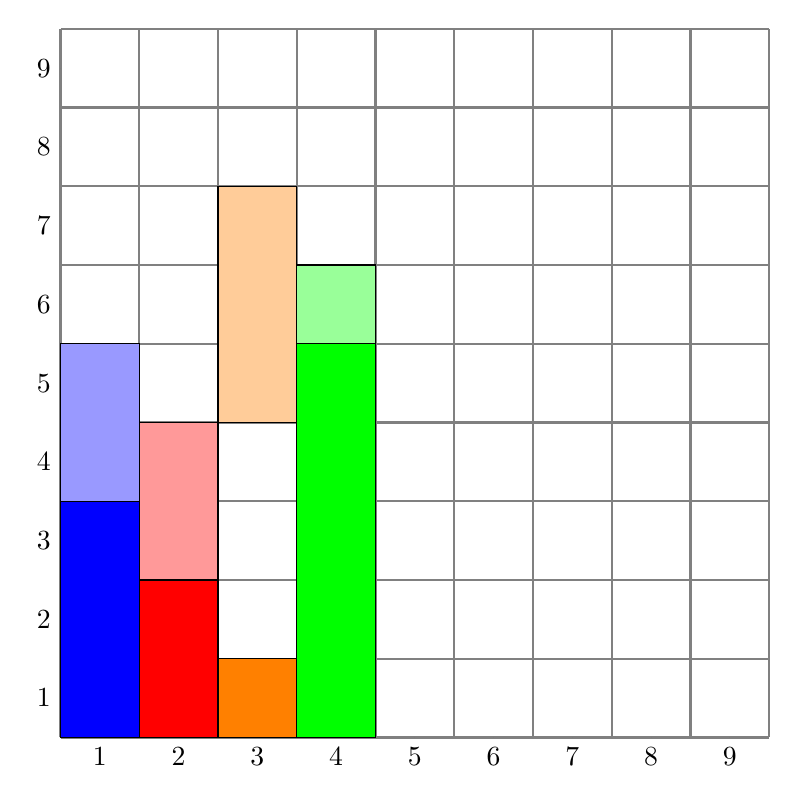
\begin{tikzpicture}
    \draw[step=1cm,gray,thick] (0.0,0.0) grid (9.0,9.0);
    
    \filldraw[black] (0.5,0) circle (0pt) node[anchor=north]{$1$};
    \filldraw[black] (1.5,0) circle (0pt) node[anchor=north]{$2$};
    \filldraw[black] (2.5,0) circle (0pt) node[anchor=north]{$3$};
    \filldraw[black] (3.5,0) circle (0pt) node[anchor=north]{$4$};
    \filldraw[black] (4.5,0) circle (0pt) node[anchor=north]{$5$};
    \filldraw[black] (5.5,0) circle (0pt) node[anchor=north]{$6$};
    \filldraw[black] (6.5,0) circle (0pt) node[anchor=north]{$7$};
    \filldraw[black] (7.5,0) circle (0pt) node[anchor=north]{$8$};
    \filldraw[black] (8.5,0) circle (0pt) node[anchor=north]{$9$};

    \filldraw[black] (0,0.5) circle (0pt) node[anchor=east]{$1$};
    \filldraw[black] (0,1.5) circle (0pt) node[anchor=east]{$2$};
    \filldraw[black] (0,2.5) circle (0pt) node[anchor=east]{$3$};
    \filldraw[black] (0,3.5) circle (0pt) node[anchor=east]{$4$};
    \filldraw[black] (0,4.5) circle (0pt) node[anchor=east]{$5$};
    \filldraw[black] (0,5.5) circle (0pt) node[anchor=east]{$6$};
    \filldraw[black] (0,6.5) circle (0pt) node[anchor=east]{$7$};
    \filldraw[black] (0,7.5) circle (0pt) node[anchor=east]{$8$};
    \filldraw[black] (0,8.5) circle (0pt) node[anchor=east]{$9$};

    \filldraw[fill=blue, draw=black] (0,0) rectangle (1,3);
    \filldraw[fill=red, draw=black] (1,0) rectangle (2,2);
    \filldraw[fill=orange, draw=black] (2,0) rectangle (3,1);
    \filldraw[fill=green, draw=black] (3,0) rectangle (4,5);

    \filldraw[fill=blue!40!white, draw=black] (0,3) rectangle (1,5);
    \filldraw[fill=red!40!white, draw=black] (1,2) rectangle (2,4);
    \filldraw[fill=orange!40!white, draw=black] (2,4) rectangle (3,7);
    \filldraw[fill=green!40!white, draw=black] (3,5) rectangle (4,6);
\end{tikzpicture}
} 
\end{center}

ตึกที่ $1$ มีความสูง $H_1=3$ แสดงโดยใช้สี \textcolor{blue}{$\blacksquare$} \\
ตึกที่ $2$ มีความสูง $H_2=2$ แสดงโดยใช้สี \textcolor{red}{$\blacksquare$} \\
ตึกที่ $3$ มีความสูง $H_3=1$ แสดงโดยใช้สี \textcolor{orange}{$\blacksquare$} \\
ตึกที่ $4$ มีความสูง $H_4=5$ แสดงโดยใช้สี \textcolor{green}{$\blacksquare$}

พื้นที่ที่สามารถวางป้อมลอยฟ้าของตึกที่ $1$ ได้ ครอบคลุมพื้นที่ตั้งแต่ $L_1=4$ ถึง $R_1=5$ แสดงโดยใช้สี \textcolor{blue!40!white}{$\blacksquare$} \\
พื้นที่ที่สามารถวางป้อมลอยฟ้าของตึกที่ $2$ ได้ ครอบคลุมพื้นที่ตั้งแต่ $L_2=3$ ถึง $R_2=4$ แสดงโดยใช้สี \textcolor{red!40!white}{$\blacksquare$} \\
พื้นที่ที่สามารถวางป้อมลอยฟ้าของตึกที่ $3$ ได้ ครอบคลุมพื้นที่ตั้งแต่ $L_3=5$ ถึง $R_3=7$ แสดงโดยใช้สี \textcolor{orange!40!white}{$\blacksquare$} \\
พื้นที่ที่สามารถวางป้อมลอยฟ้าของตึกที่ $4$ ได้ ครอบคลุมพื้นที่ตั้งแต่ $L_4=6$ ถึง $R_4=6$ แสดงโดยใช้สี \textcolor{green!40!white}{$\blacksquare$} \\

โดยสามารถวางป้อมลอยฟ้าได้ทั้งหมด $9$ แบบ ได้แก่
\begin{enumerate}
    \item ไม่วางในช่องใด ๆ
    \item วางในช่อง $(1,4)$
    \item วางในช่อง $(1,5)$
    \item วางในช่อง $(2,3)$
    \item วางในช่อง $(2,4)$
    \item วางในช่อง $(3,5)$
    \item วางในช่อง $(3,6)$
    \item วางในช่อง $(3,7)$
    \item วางในช่อง $(4,6)$
\end{enumerate}

\pagebreak

คำอธิบายตัวอย่างที่ 2 \\
\begin{center}
\parindent \resizebox{5cm}{!}{
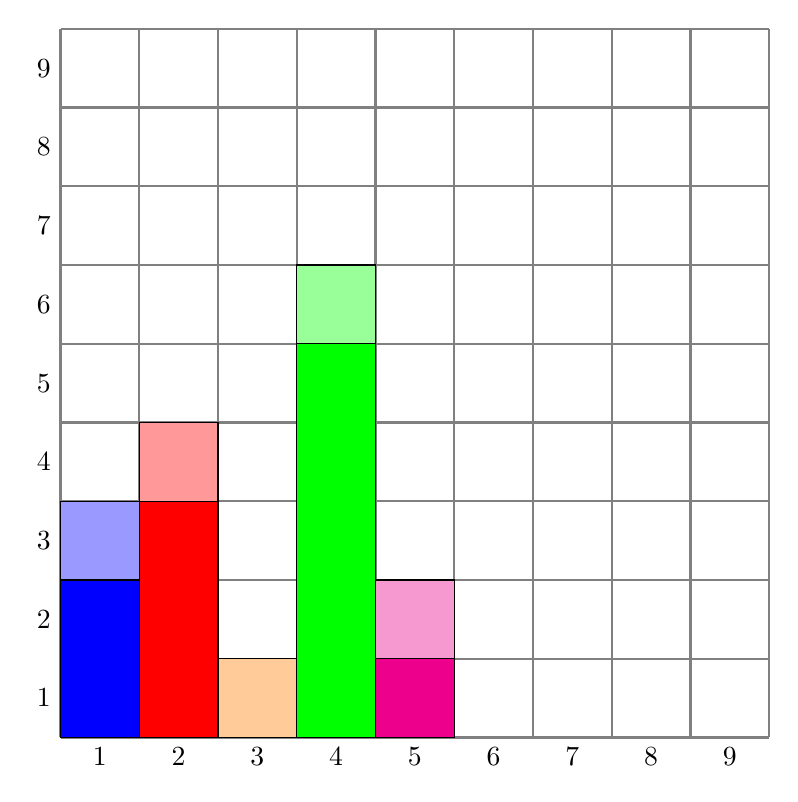
\begin{tikzpicture}
    \draw[step=1cm,gray,thick] (0.0,0.0) grid (9.0,9.0);
    
    \filldraw[black] (0.5,0) circle (0pt) node[anchor=north]{$1$};
    \filldraw[black] (1.5,0) circle (0pt) node[anchor=north]{$2$};
    \filldraw[black] (2.5,0) circle (0pt) node[anchor=north]{$3$};
    \filldraw[black] (3.5,0) circle (0pt) node[anchor=north]{$4$};
    \filldraw[black] (4.5,0) circle (0pt) node[anchor=north]{$5$};
    \filldraw[black] (5.5,0) circle (0pt) node[anchor=north]{$6$};
    \filldraw[black] (6.5,0) circle (0pt) node[anchor=north]{$7$};
    \filldraw[black] (7.5,0) circle (0pt) node[anchor=north]{$8$};
    \filldraw[black] (8.5,0) circle (0pt) node[anchor=north]{$9$};

    \filldraw[black] (0,0.5) circle (0pt) node[anchor=east]{$1$};
    \filldraw[black] (0,1.5) circle (0pt) node[anchor=east]{$2$};
    \filldraw[black] (0,2.5) circle (0pt) node[anchor=east]{$3$};
    \filldraw[black] (0,3.5) circle (0pt) node[anchor=east]{$4$};
    \filldraw[black] (0,4.5) circle (0pt) node[anchor=east]{$5$};
    \filldraw[black] (0,5.5) circle (0pt) node[anchor=east]{$6$};
    \filldraw[black] (0,6.5) circle (0pt) node[anchor=east]{$7$};
    \filldraw[black] (0,7.5) circle (0pt) node[anchor=east]{$8$};
    \filldraw[black] (0,8.5) circle (0pt) node[anchor=east]{$9$};

    \filldraw[fill=blue, draw=black] (0,0) rectangle (1,2);
    \filldraw[fill=red, draw=black] (1,0) rectangle (2,3);
    \filldraw[fill=orange, draw=black] (2,0) rectangle (3,0);
    \filldraw[fill=green, draw=black] (3,0) rectangle (4,5);
    \filldraw[fill=magenta, draw=black] (4,0) rectangle (5,1);

    \filldraw[fill=blue!40!white, draw=black] (0,2) rectangle (1,3);
    \filldraw[fill=red!40!white, draw=black] (1,3) rectangle (2,4);
    \filldraw[fill=orange!40!white, draw=black] (2,0) rectangle (3,1);
    \filldraw[fill=green!40!white, draw=black] (3,5) rectangle (4,6);
    \filldraw[fill=magenta!40!white, draw=black] (4,1) rectangle (5,2);
\end{tikzpicture}
} 
\end{center}

ตึกที่ $1$ มีความสูง $H_1=2$ แสดงโดยใช้สี \textcolor{blue}{$\blacksquare$} \\
ตึกที่ $2$ มีความสูง $H_2=3$ แสดงโดยใช้สี \textcolor{red}{$\blacksquare$} \\
ตึกที่ $3$ มีความสูง $H_3=0$ แสดงโดยใช้สี \textcolor{orange}{$\blacksquare$} \\
ตึกที่ $4$ มีความสูง $H_4=5$ แสดงโดยใช้สี \textcolor{green}{$\blacksquare$} \\
ตึกที่ $5$ มีความสูง $H_5=1$ แสดงโดยใช้สี \textcolor{magenta}{$\blacksquare$}

พื้นที่ที่สามารถวางป้อมลอยฟ้าของตึกที่ $1$ ได้ ครอบคลุมพื้นที่ตั้งแต่ $L_1=3$ ถึง $R_1=3$ แสดงโดยใช้สี \textcolor{blue!40!white}{$\blacksquare$} \\
พื้นที่ที่สามารถวางป้อมลอยฟ้าของตึกที่ $2$ ได้ ครอบคลุมพื้นที่ตั้งแต่ $L_2=4$ ถึง $R_2=4$ แสดงโดยใช้สี \textcolor{red!40!white}{$\blacksquare$} \\
พื้นที่ที่สามารถวางป้อมลอยฟ้าของตึกที่ $3$ ได้ ครอบคลุมพื้นที่ตั้งแต่ $L_3=1$ ถึง $R_3=1$ แสดงโดยใช้สี \textcolor{orange!40!white}{$\blacksquare$} \\
พื้นที่ที่สามารถวางป้อมลอยฟ้าของตึกที่ $4$ ได้ ครอบคลุมพื้นที่ตั้งแต่ $L_4=6$ ถึง $R_4=6$ แสดงโดยใช้สี \textcolor{green!40!white}{$\blacksquare$} \\
พื้นที่ที่สามารถวางป้อมลอยฟ้าของตึกที่ $5$ ได้ ครอบคลุมพื้นที่ตั้งแต่ $L_5=2$ ถึง $R_5=2$ แสดงโดยใช้สี \textcolor{magenta!40!white}{$\blacksquare$} \\

โดยสามารถวางป้อมลอยฟ้าได้ทั้งหมด $11$ แบบ ได้แก่
\begin{enumerate}
    \item ไม่วางในช่องใด ๆ
    \item วางในช่อง $(1,3)$
    \item วางในช่อง $(2,4)$
    \item วางในช่อง $(3,1)$
    \item วางในช่อง $(4,6)$
    \item วางในช่อง $(5,2)$
    \item วางในช่อง $(1,3)$ และ $(3,1)$
    \item วางในช่อง $(1,3)$ และ $(5,2)$
    \item วางในช่อง $(2,4)$ และ $(5,2)$
    \item วางในช่อง $(3,1)$ และ $(5,2)$
    \item วางในช่อง $(1,3)$, $(3,1)$ และ $(5,2)$
\end{enumerate}

\end{problem}

\end{document}
